% ARCHITECTURE
\chapter{Architecture}\label{chapter:architecture}

% General architecture of the application
% central server with API and three mobile apps
% MVC REST API to mobile App
% MVC in the App's internal structure

%First we will discuss how the different components of the application's architecture are combined and communicate. Next we will give an overview of the how the data is structured. Finally we will look at each app in more detail.

% Architectural paradigms
%	Data organization and mobile computing
%
% heterogeneity also apparent in mobile apps themselves
%		(software : html5 vs android vs ios)
%		(performance : native vs web)
%		(hardware : e.g. android has to deal with different screen sizes)

% mobile computing
% Stefan Ternier proposes \cite{ternier:2012}

\section{Architectural challenges}

Before discussing the end result, we will try to give an overview of some of the challenges that need to be addressed when designing mobile applications. One of the central questions when building any application is how to organize information. Trade-offs in the design of data organization go beyond the level of the data itself. For example the physical location of data, i.e., whether data is kept locally or stored remotely. Availability, fault-tolerance and Quality of service (Qos), which covers reliability, security and performance, are other aspects that can be taken into account\cite{}.

To support interactions between users on different devices, some data will be sent over the network. Several communication paradigms exist, such as direct or indirect communication. The important difference here is that in the second case an additional layer of indirection exists, decoupling the producers and consumers of information streams\cite{coulouris:2012}. These communicating entities can also take on different roles, from a \emph{client-server} approach were clients are consumers and servers are producers, to a \emph{peer-to-peer} (P2P) architecture where conceptually only one type of role exists\cite{coulouris:2012}.

In a distributed environment software engineers may have to deal with a degree of heterogeneity both in software and hardware. As a result layers of transparency can be introduced to reduce complexity of the underlying structures.

Another challenge of the application that we are building is inherent to \emph{mobile computing}. Coulouris et al. define mobile computing as "the performance of computing tasks while the user is on the move, or visiting places other than their usual environment"\cite{coulouris:2012}. This poses a difficulty, as the quality of the connection may fluctuate, devices may be disconnected and reconnected as the user moves, or temporary go offline for an undefined period of time\cite{coulouris:2012}. Although this is an important aspect, it is not a major concern of the application as changes in the data may take several minutes to hours or days to take place. However, when creating data, it might be a good idea to give an option to store local drafts; for example when the connection is lost.


\section{Architecture design}

The roles of the communicating entities correspond to the client-server paradigm. The choice for this architecture is to provide a single point to access stored data. Storing all data locally and exchanging updates is possible, but would be a lot more complicated. Based on the characteristics of peer-to-peer systems, replication, CPU usage, and network traffic, introduce significant constraints on the mobile device's performance. Bandwidth, local storage and CPU are all much more limited than in home computers. In addition, due to their mobile nature, the physical layout of the network may change constantly. As a result, a client-server approach seems the logical choice. The global architecture is shown in figure \ref{figure:architecture:global}.

\begin{figure}
	
	\begin{center}
		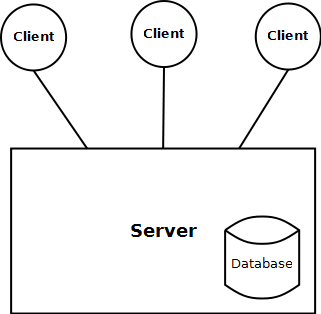
\includegraphics[width=200px]{img/architecture_global}
		\caption{The global architecture of the application.}
		\label{figure:architecture:global}
	\end{center}

\end{figure}

To allow access to the database, each application can talk to a public interface. For example, in listing \ref{listing:dbaccess} is shown how one could use \texttt{PHP} scripts to access the database, using URLs to pass arguments. This kind of approach is 

%% LISTING
%\lstinputlisting[language=PHP, caption={Example of a \texttt{PHP} script to insert data into the database (simplification).}, label={listing:dbaccess}]{code/dbaccess.php}

In this case, REST (Representational State Transfer) was used to implement this point of public access. The REST approach uses \texttt{HTTP} operations GET, PUT, DELETE and POST to manipulate resources represented in XML\cite{coulouris:2012}. The API shields the underlying data structures from the clients, organizes the application's data model into resources and can be accessed through a standardized protocol.

The REST API used here, consists out of a series of methods, as listed in table \ref{table:rest_api}. Five resources are provided: \emph{answer}, \emph{authentication}, \emph{question}, \emph{skill}, and \emph{user}.



\begin{table}
	\caption{REST API}\label{table:rest_api}
	
	\begin{center}
		\begin{tabular}{p{70px} | p{70px} | p{210px}}
				\hline
				\hline
				\textbf{Resource} 		& \textbf{Method}					&	\textbf{Description} 	\\
				\hline
				\hline
				\texttt{ANSWER}				& 												&	\\
				\hline
															& \emph{create}						& Create a new answer. \\
															& \emph{get\_question}		& Get the question this answer was posted on. \\
															%& \emph{search}						& Search an answer.	\\
				\hline
				\texttt{AUTHENTICATION}		& 												&	\\
				\hline
															& \emph{endsession}				& Create a new answer. \\
															& \emph{startsession}			& Get the question this answer was posted on. \\
				\hline
				\texttt{QUESTION}			& 												& \\
				\hline
															& \emph{create}						& Post a new question. \\
															& \emph{get\_answers}			& Get the answers for a question. \\
															& \emph{get\_info}				& Get information on a question. \\
															& \emph{get\_skills}			& Get the skills related to this question. \\
															& \emph{remove}						& Delete a question. \\
															%& \emph{search}						& Search questions, given a number of search parameters. \\
				\hline
				\texttt{SKILL}				& 												& \\
				\hline
															& \emph{create}						& Create a new skill and add it to the database. \\
															& \emph{get\_questions}		& Get questions related to a given skill. \\
															%& \emph{search}						& Search skills. \\
				\hline
				\texttt{USER}					&	\\
				\hline
															& \emph{get\_answers}			& Get the answers submitted by a user. \\
															& \emph{get\_questions}		& Get questions submitted by a user. \\
															& \emph{get\_info}				&	Retrieve profile information about a user.	\\
															& \emph{get\_skills}			& Get the skills of a user. \\
															& \emph{register}					&	Register a new user account. \\
															& \emph{search}						&	Search a user given certain parameters. \\
															& \emph{unregister}				&	Delete a user account. \\
															& \emph{update\_info}			& Update profile information about a user. \\
															%& \emph{getContacts}	  	& \\
															%& \emph{}									& \\
				\hline
				\hline
		\end{tabular}
	\end{center}
	
\end{table}

